% Copyright © 2015-2016 Martin Ueding <dev@martin-ueding.de>
%
\documentclass[english, fleqn]{beamer}


\usetheme{Malmoe}
\useoutertheme{infolines}
\usepackage[bibatend]{header}

\newcommand\qqandqq{\qquad\text{and}\qquad}

\DeclareMathOperator\Span{Span}

\DeclareSIUnit\year{yr}

\AtBeginSection[]
{
    \begin{frame}
        \sectionpage
        \tableofcontents[
            sectionstyle=show/shaded,
            subsectionstyle=hide/hide/hide,
            subsubsectionstyle=hide/hide/hide
        ]
    \end{frame}
}

\AtBeginSubsection[]
{
    \begin{frame}
        \subsectionpage
        \tableofcontents[
            sectionstyle=show/hide,
            subsectionstyle=show/shaded/hide,
            subsubsectionstyle=hide/hide/hide
        ]
    \end{frame}
}

\colorlet{qred}{red!85!black}
\colorlet{qgreen}{green!85!black}
\colorlet{qblue}{blue!85!black}

\renewcommand\iup{\text i}
\renewcommand\eup{\text e}

%\setbeamersize{text margin left=2.5em}
\setbeamertemplate{bibliography item}[text]


\setbeamertemplate{navigation symbols}{}
%\addtobeamertemplate{navigation symbols}{}{%
%    \usebeamerfont{footline}%
%    \usebeamercolor[fg]{footline}%
%    \hspace{1em}%
%    \insertframenumber/\inserttotalframenumber
%}

\graphicspath{{_build/}{Figures/}}

\title{Nucleon Decay}
%\subtitle{}
\author{Martin Ueding -- mu@martin-ueding.de}
%\date{}

\begin{document}

\begin{frame}
    \titlepage
\end{frame}

\begin{frame}
    \titlepage
\end{frame}

\section{Standard model}

\begin{frame}
    \frametitle{Standard model}

    \begin{columns}[t]
        \begin{column}{.3\linewidth}
            \begin{block}{Fermions}
                \

                \begin{tabular}{ccc}
                    u & c & t \\
                    d & s & b \\
                    \midrule
                    $\nuup_\mathsf e$ & $\nuup_\muup$ & $\nuup_\tauup$ \\
                    $\mathsf e^-$ & $ \muup^-$ & $\tauup^-$
                \end{tabular}
            \end{block}
        \end{column}
        \begin{column}{.7\linewidth}
            \begin{block}{Bosons}
                \

                \begin{tabular}{llll}
                    Group & Force & Property & Carrier \\
                    \midrule
                    $\mathsf{SU}(3)$ & Strong & Color & Gluon \\
                    $\mathsf{SU}(2)$ & Weak & Weak Isospin & W, Z \\
                    $\mathsf{SU}(1)$ & EM & Hypercharge & B, $\gammaup$
                \end{tabular}
            \end{block}
        \end{column}
    \end{columns}

    \

    \begin{block}{Gauge group}
        $\mathsf{SU}(3) \times \mathsf{SU}(2) \times \mathsf{SU}(1)$
    \end{block}

\end{frame}

\section{Grand unified theories}

\subsection{Motivation}

\begin{frame}
    \frametitle{Charges}

    Quarks and leptons electric charges are very related:
    \[
        \frac{Q(\mathsf u)}{Q(\mathsf e^+)} = \frac 23
        \qqandqq
        \frac{Q(\mathsf d)}{Q(\mathsf e^+)} = - \frac 13
    \]

    \pause

    And most strikingly:
    \[
        \frac{Q(\mathsf p)}{Q(\mathsf e^+)} = 1
    \]

    \pause

    \begin{itemize}
        \item QED does not need this
        \item Begs for unification
        \item Be careful with anthropic principle!
    \end{itemize}
\end{frame}

\begin{frame}
    \frametitle{Number of particles}

    \begin{itemize}
        \item Two quarks per generation
        \item Two leptons per generation
        \item Three generations of quarks and leptons
    \end{itemize}
\end{frame}

\begin{frame}
    \frametitle{Running of the coupling}
    \framesubtitle{The familiar graph}

    {
        \centering
        \includegraphics{running}
    }

    \parencite{Peskin/1997ez}
\end{frame}

\begin{frame}
    \frametitle{Running of the coupling}
    \framesubtitle{Where it comes from}

    \includegraphics{loop} 

    \

    \includegraphics{loop2} 
\end{frame}

\begin{frame}
    \frametitle{Running of the coupling}
    \framesubtitle{The familiar graph (again)}

    {
        \centering
        \includegraphics{running}
    }

    \parencite{Peskin/1997ez}
\end{frame}

\begin{frame}
    % TODO Does this really apply?

    \frametitle{Matter and anti-matter asymmetry}

    Why is there more matter than anti-matter?

    Standard model is symmetric

    Violation via GUT process?
\end{frame}

\subsection{Lie algebras}

\begin{frame}
    \frametitle{Lie group}

    \begin{itemize}
        \item A continuous symmetry group
        \item Matrix groups like SU($N$), SO($N$), GL, SL
        \item Fundamental representation
        \item Manifold structure
        \item Algebra and tangent space
    \end{itemize}

\end{frame}

\begin{frame}
    \frametitle{Group representation}
    \framesubtitle{Definition}

    \begin{itemize}
        \item Representation $D^\Gamma$ maps group elements to linear operators
        \item Not necessarily faithful
        \item Multiple representations $\Gamma$ possible
    \end{itemize}

    \

    \begin{center}
        \includegraphics{representation}
    \end{center}
\end{frame}

\begin{frame}
    \frametitle{Group representation}
    \framesubtitle{Example}
    
    \begin{columns}
        \begin{column}{.6\linewidth}
            Take group SO(2). Represent on $\R^3$:
            \[
                D(g_\phi) =
                \begin{pmatrix}
                    \cos(\phi) & - \sin(\phi) & 0 \\
                    \sin(\phi) & \cos(\phi) & 0 \\
                    0 & 0 & 1
                \end{pmatrix}
            \]

            Acts on $(x, y, z)^\mathsf T \in \R^3$
        \end{column}
        \pause
        \begin{column}{.4\linewidth}
            \begin{itemize}
                \item $\{ x, y \}$ is a doublet
                \item $\{ z \}$ is a singlet
                \item Representation is reducible
            \end{itemize}
        \end{column}
    \end{columns}
\end{frame}

\begin{frame}
    \frametitle{Group representation}
    \framesubtitle{Standard model}

    \begin{columns}[t]
        \begin{column}{.55\textwidth}

            \begin{itemize}
                \item Color, SU(3) is represented on $\C^3$
                \item Weak isospin, SU(2) on $\C^2$
            \end{itemize}

            Can we combine that to $\C^5$?

            \pause

            We can! Let $C \in \mathsf{SU}(3)$ and $W \in \mathsf{SU}(2)$.
            \pause
            \[
                \begin{pmatrix}
                    W & 0 \\
                    0 & 1
                \end{pmatrix}
                \qqandqq
                \begin{pmatrix}
                    1 & 0 \\
                    0 & C
                \end{pmatrix}
            \]

            Acts on $(\nuup_\mathsf L, \mathsf e^-_\mathsf L,
            \bar{\textcolor{qred}{\mathsf d}}_\mathsf L,
            \bar{\textcolor{qgreen}{\mathsf d}}_\mathsf L,
            \bar{\textcolor{qblue}{\mathsf d}}_\mathsf L)^\mathsf T$.
        \end{column}
        \pause
        \begin{column}{.45\textwidth}
            \begin{itemize}
                \item Lepton part doublet under $W$.
                \item Quark part \enquote{trivial} under $W$.
                \item Lepton part trivial under $C$.
                \item Quark part triplet under $C$.
                \item Reducible into irreps
            \end{itemize}
        \end{column}
    \end{columns}
\end{frame}

\begin{frame}
    \frametitle{Irreps used in the Standard model}

    Which $\mathsf U(1) \times \mathsf{SU}(2) \times \mathsf{SU}(3)$ irrep do the particles belong to?

    \begin{tabular}{lcc}
        \toprule
        Name & Particles & Irrep \\
        \midrule
        L leptons &
        $\begin{pmatrix}
            \nuup_\mathsf L \\
            \eup^-_\mathsf L
        \end{pmatrix}$ &
        $\setname C_{-1} \otimes \setname C^2 \otimes \setname C$ \\
        L quarks &
        $\begin{pmatrix}
            \textcolor{qred}{\mathsf u}_\mathsf L &
            \textcolor{qgreen}{\mathsf u}_\mathsf L &
            \textcolor{qblue}{\mathsf u}_\mathsf L \\
            \textcolor{qred}{\mathsf d}_\mathsf L &
            \textcolor{qgreen}{\mathsf d}_\mathsf L &
            \textcolor{qblue}{\mathsf d}_\mathsf L
        \end{pmatrix}$ &
        $\setname C_{-1/3} \otimes \setname C^2 \otimes \setname C^3$ \\
        R neutrino &
        $\nuup_\mathsf R$ &
        $\setname C_{0} \otimes \setname C \otimes \setname C$ \\
        R electron &
        $\eup_\mathsf R$ &
        $\setname C_{-2} \otimes \setname C \otimes \setname C$ \\
        R up quarks &
        $\begin{pmatrix}
            \textcolor{qred}{\mathsf u}_\mathsf R &
            \textcolor{qgreen}{\mathsf u}_\mathsf R &
            \textcolor{qblue}{\mathsf u}_\mathsf R
        \end{pmatrix}$ &
        $\setname C_{4/3} \otimes \setname C \otimes \setname C^3$ \\
        R down quarks &
        $\begin{pmatrix}
            \textcolor{qred}{\mathsf d}_\mathsf R &
            \textcolor{qgreen}{\mathsf d}_\mathsf R &
            \textcolor{qblue}{\mathsf d}_\mathsf R
        \end{pmatrix}$ &
        $\setname C_{-2/3} \otimes \setname C \otimes \setname C^3$ \\
        \bottomrule
    \end{tabular}

    \

    $\C_Y$ defined via $\alpha \cdot \C_Y = \alpha^{3Y} \C_Y$
\end{frame}

\begin{frame}
    \frametitle{Fermion representation}

    Introduce the Fermion representation
    \begin{align*}
        F &:= 
        \setname C_{-1} \otimes \setname C^2 \otimes \setname C
        \quad\oplus\quad \setname C_{-1/3} \otimes \setname C^2 \otimes \setname C^3
        \quad\oplus\quad \setname C_{0} \otimes \setname C \otimes \setname C
        \\&\qquad\oplus\quad \setname C_{-2} \otimes \setname C \otimes \setname C
        \quad\oplus\quad \setname C_{4/3} \otimes \setname C \otimes \setname C^3
        \quad\oplus\quad \setname C_{-2/3} \otimes \setname C \otimes \setname C^3
    \end{align*}

    \pause

    Standard model representation is $F \oplus F^*$.
\end{frame}

\subsection{Georgi-Glashow model}

\begin{frame}
    \frametitle{Extension to SU(5)}
    \begin{block}{The quest}
        From $\mathsf{SU}(3) \times \mathsf{SU}(2) \times \mathsf U(1)$ to $\mathsf{SU}(5)$.
    \end{block}

    \begin{block}{Dimensionality}
        \begin{itemize}
            \item $\mathsf{SU}(N)$ has dimension $N^2 - 1$
            \item Standard model has $8 \cdot 3 \cdot 1 = 24$ dimensions
            \item SU(5) has 24 dimensions
        \end{itemize}

        So far, so good
    \end{block}
\end{frame}

\begin{frame}
    \frametitle{Digital code}

    \begin{columns}[t]
        \begin{column}{0.5\linewidth}
            \begin{itemize}
                \item
                    $F \oplus F^*$ has $32 = 2^5$ dimensions.
                \pause
                \item
                    Introduce a bit code:
                    \begin{enumerate}
                        \item Isospin up
                        \item Isospin down
                        \item \textcolor{qred}{Red}
                        \item \textcolor{qgreen}{Green}
                        \item \textcolor{qblue}{Blue}
                    \end{enumerate}
                \item
                    Binary complement shall be antiparticle
            \end{itemize}
        \end{column}
        \pause
        \begin{column}{0.5\linewidth}
            \begin{exampleblock}{Example}
                \begin{itemize}
                    \item 01100, down and red: $\textcolor{qred}{\mathsf d}_\mathsf L$
                    \item 10011, up and green-blue: $\bar{\textcolor{qred}{\mathsf d}}_\mathsf R$
                    \item 10111, up: $\eup^-_\mathsf L$
                    \item 00010, green: $\textcolor{qgreen}{\mathsf d}_\mathsf R$
                    \item 00000: $\bar\nuup_\mathsf L$ or $\nuup_\mathsf R$
                \end{itemize}
            \end{exampleblock}
        \end{column}
    \end{columns}
\end{frame}

\begin{frame}
    \frametitle{Exterior algebra}

    \begin{block}{Idea}
        Represent bit-code on exterior algebra $\Lambda \C^5$
    \end{block}

    \pause

    \begin{block}{Implementation}
        \begin{itemize}
            \item Five properties are basis 1-forms: $u$, $d$, $r$, $g$, $b$
            \item Algebra:
                \begin{itemize}
                    \item $u \wedge d := u \otimes d - d \otimes u$
                    \item $u \wedge u = 0$
                    \item $u \wedge d = - d \wedge u$
                \end{itemize}
            \item
                $\Lambda C^5 = 
                \Lambda^0 \C^5
                \oplus \Lambda^1 \C^5
                \oplus \Lambda^2 \C^5
                \oplus \Lambda^3 \C^5
                \oplus \Lambda^4 \C^5
                \oplus \Lambda^5 \C^5$
        \end{itemize}
    \end{block}
\end{frame}

\begin{frame}
    \frametitle{Isospin and color splitting}

    \begin{itemize}
        \item Our choice of properties implies $\C^2 \oplus \C^3$ splitting
        \pause
        \item We describe $\mathsf S(\mathsf U(2) \times \mathsf U(3))$
        \pause
        \item This is isomorphic to $G_\text{SM}$, modulo finite subgroup
    \end{itemize}

    \pause

    \begin{alertblock}{What about U(1)?}
        \begin{itemize}
            \item Not easy to include in $\C^5$
            \item U(1) is factor in $G_\text{SM}$, must commute with $\mathsf S(\mathsf U(2) \times \mathsf U(3))$
        \end{itemize}
    \end{alertblock}

    \pause

    \begin{block}{Schur's lemma}
        Only a multiple of unit matrix commutes with every matrix in an irrep.
    \end{block}
\end{frame}

\begin{frame}
    \frametitle{Using Schur's lemma}

    \begin{columns}[t]
        \begin{column}{.5\textwidth}
            \begin{block}{First try}
                Represent U(1) with
                \[
                    \begin{pmatrix}
                        \alpha &&&& \\
                        & \alpha &&& \\
                        && \beta && \\
                        &&& \beta & \\
                        &&&& \beta
                    \end{pmatrix}
                \]

                Is not unitary for $\alpha, \beta \in \C$.
            \end{block}
        \end{column}
        \begin{column}{.5\textwidth}
            \begin{block}{Second try}
                Need $\alpha^2 \beta^3 = 1$. Use
                \[
                    \begin{pmatrix}
                        \alpha^3 &&&& \\
                        & \alpha^3 &&& \\
                        && \alpha^{-2} && \\
                        &&& \alpha^{-2} & \\
                        &&&& \alpha^{-2}
                    \end{pmatrix}
                \]
                
                That is unitary for any $\alpha \in \C$.
            \end{block}
        \end{column}
    \end{columns}
\end{frame}

\begin{frame}
    \frametitle{Group isomorphism}

    Our group mapping currently is:
    \[
        \begin{array}{lccc}
            \phi\colon & \mathsf{U}(1) \times \mathsf{SU}(2) \times \mathsf{SU}(3) & \to & \mathsf{SU}(5) \\
            & (\alpha, g, h) & \mapsto &
            \begin{pmatrix}
                \alpha^3 g & 0 \\
                0 & \alpha^{-2} h
            \end{pmatrix}
        \end{array}
    \]

    \pause

    \begin{block}{Is that an isomorphism?}
        \begin{itemize}
            \item No, it has a kernel $(\alpha, \alpha^{-3}, \alpha^2)$.
            \item For $\alpha^6 = 1$ we have $\alpha^{-3} \in \mathsf{SU}(2)$ and $\alpha^{2} \in \mathsf{SU}(3)$
            \item That is a $\setname Z_6$ kernel (finite group).
        \end{itemize}
    \end{block}
\end{frame}

\begin{frame}
    \frametitle{The crucial trial}

    Can we really reduce U(1) to $\setname Z_6$?

    For $\alpha \in \mathsf U(1)$ it acts as $(\alpha, \alpha^{-3}, \alpha^2)$.

    We need:

    \begin{tabular}{lcc}
        \toprule
        Name & Representation & Relation \\
        \midrule
        L quark &
        $\setname C_{Y} \otimes \setname C^2 \otimes \setname C^3$ &
        $\alpha^{3Y -3 +2} = 1$ \\
        L lepton &
        $\setname C_{Y} \otimes \setname C^2 \otimes \setname C$ &
        $\alpha^{3Y -3} = 1$ \\
        R quark &
        $\setname C_{Y} \otimes \setname C \otimes \setname C^3$ &
        $\alpha^{3Y +2} = 1$ \\
        R lepton &
        $\setname C_{Y} \otimes \setname C \otimes \setname C$ &
        $\alpha^{3Y} = 1$ \\
        \bottomrule
    \end{tabular}
\end{frame}

\begin{frame}
    \frametitle{The crucial trial}
    
    \begin{tabular}{lrll}
        \toprule
        Name & Relation & Hypercharge & Actual \\
        \midrule
        L quark & $3Y -1 \in 6 \Z$ & $Y = \text{even integer} + 1/3$ & $Y = 1/3$ \\
        L lepton & $3Y -3 \in 6 \Z$ & $Y = \text{odd integer}$ & $Y = -1$ \\
        R quark & $3Y +2 \in 6 \Z$ & $Y = \text{odd integer} + 1/3$ & $Y_\mathsf u = 4/3$, $Y_\mathsf d = -2/3$ \\
        R lepton & $3Y \in 6 \Z$ & $Y = \text{even integer}$ & $Y = -2$ \\
        \bottomrule
    \end{tabular}

    \

    \pause

    It works!
    \[
        G_\text{SM} / \Z^6 \simeq \mathsf S(\mathsf U(2) \times \mathsf U(3)) \subset \mathsf{SU}(5)
    \]

    We have a group isomorphism
\end{frame}

\begin{frame}
    \frametitle{Irreducible representations of SU(5)}
    \framesubtitle{Overview}

    How to represent $F \oplus F^*$ on SU(5)?

    \

    Exterior algebra:
    \[
        \Lambda C^5 = 
                \Lambda^0 \C^5
                \oplus \Lambda^1 \C^5
                \oplus \Lambda^2 \C^5
                \oplus \Lambda^3 \C^5
                \oplus \Lambda^4 \C^5
                \oplus \Lambda^5 \C^5
    \]

    Dimensions:
    \[
        32 = 1 + 5 + 10 + 10 + 5 + 1
    \]
\end{frame}

\begin{frame}
    \frametitle{Irreducible representations of SU(5)}
    \framesubtitle{Zeroth one}

    Easiest ones: $\Lambda^0 \C^5 \simeq \C$ and $\Lambda^5 \C^5 \simeq \C$

    One dimensional singlets.

    We could do
    \begin{align*}
        \Lambda^0 \C^5 &= \Span(\nuup_\mathsf R) \\
        \Lambda^5 \C^5 &= \Span(\bar \nuup_\mathsf L) \,,
    \end{align*}
    or the other way around.
\end{frame}

\begin{frame}
    \frametitle{Irreducible representations of SU(5)}
    \framesubtitle{First one}

    Next one: $\Lambda^1 \C^5 \simeq \C^5$

    \begin{itemize}
        \item 

    
    This space is acted upon with
    \[
            \phi\colon 
             (\alpha, g, h)  \mapsto
            \begin{pmatrix}
                \alpha^3 g & 0 \\
                0 & \alpha^{-2} h
            \end{pmatrix}
    \]


    \item
        Preservation of $\C^2$ and $\C^3$ splitting
    \item
        $\C^2$ part transforms as $Y = 1$ in U(1), fundamentally under SU(2)
        and trivially under SU(3). Left-handed lepton with $Y = 1$.
    \item
        No such lepton. Self-dual fundamental SU(2) representation. Right-handed anti-lepton with $Y = 1$.
    \item
        $\C^3$ part transforms as $Y = - 2/3$ in U(1), trivially under
        SU(2) and fundamentally under SU(3). Right-handed down quark.
    \end{itemize}
\end{frame}

\begin{frame}
    \frametitle{Irreducible representations of SU(5)}
    \framesubtitle{First one}

    $\Lambda^1 \C^5 \simeq \C^5$ describes:
    \begin{itemize}
        \item $\mathsf e^+_\mathsf R$
        \item $\bar\nuup_\mathsf R$
        \item $\textcolor{qred}  {\mathsf d}_\mathsf R$
        \item $\textcolor{qgreen}{\mathsf d}_\mathsf R$
        \item $\textcolor{qblue} {\mathsf d}_\mathsf R$
    \end{itemize}

    \

    As spaces:
    $\C^5 \simeq \C_1 \otimes \C^2 \otimes \C \quad\oplus\quad \C_{-2/3} \otimes \C \otimes \C^3$
\end{frame}

\begin{frame}
    \frametitle{Irreducible representations of SU(5)}
    \framesubtitle{Second one}

    \begin{itemize}
        \item Look at $\Lambda^2 \C^5$
        \item Know already that $\C^5 \simeq \C_1 \otimes \C^2 \otimes \C \quad\oplus\quad \C_{-2/3} \otimes \C \otimes \C^3$
        \item Use $\Lambda^2(V \oplus W) \simeq \Lambda^2 V \oplus (V \otimes W) \oplus \Lambda^2 W$
    \end{itemize}

        We obtain
            \begin{align*}
                \Lambda^2 \C^5
                &\simeq
                \Lambda^2(\C_1 \otimes \C^2 \otimes \C \quad\oplus\quad \C_{-2/3} \otimes \C \otimes \C^3) \\
                &\simeq
                \Lambda^2(\C_1 \otimes \C^2 \otimes \C)
                \\&\quad\oplus\quad 
                (\C_1 \otimes \C^2 \otimes \C) \otimes (\C_{-2/3} \otimes \C \otimes \C^3)
                \\&\quad\oplus\quad 
                \Lambda^2(\C_{-2/3} \otimes \C \otimes \C^3)
            \end{align*}
\end{frame}

\begin{frame}
    \frametitle{Irreducible representations of SU(5)}
    \framesubtitle{Second one}

    \begin{tabular}{lll}
        \toprule
        Summand & Isomorphic to & Particles \\
        \midrule
        $\Lambda^2(\C_1 \otimes \C^2 \otimes \C)$ & $\C_2 \otimes \C \otimes \C$ & $\mathsf e^+_\mathsf L$ \\
        $(\C_1 \otimes \C^2 \otimes \C) \otimes (\C_{-2/3} \otimes \C \otimes \C^3)$ & $\C_{1/3} \otimes \C^2 \otimes \C^3$ & $\mathsf u_\mathsf L$ and $\mathsf d_\mathsf L$ \\
        $\Lambda^2(\C_{-2/3} \otimes \C \otimes \C^3)$ & $\C_{-4/3} \otimes \C \otimes \C^3$ & $\bar{\mathsf u}_\mathsf L$ \\
        \bottomrule
    \end{tabular}
\end{frame}

\begin{frame}
    \frametitle{Irreducible representations of SU(5)}
    \framesubtitle{Last three ones}

    \begin{itemize}
        \item 
            Still have $\Lambda^3 \C^5$, $\Lambda^4 \C^5$ and $\Lambda^5 \C^5$
        \item
            Those are Hodge-Dual to the others
        \item
            Hodge-Dual corresponds to binary complement
        \item
            Binary complement is anti-particle
    \end{itemize}
\end{frame}

\begin{frame}
    \frametitle{Multiplets of SU(5)}

    \begin{tabular}{*6c}
        \toprule
        $\Lambda^0 \C^5$ &
        $\Lambda^1 \C^5$ &
        $\Lambda^2 \C^5$ &
        $\Lambda^3 \C^5$ &
        $\Lambda^4 \C^5$ &
        $\Lambda^5 \C^5$ \\
        \midrule
        $\begin{pmatrix}
            \bar\nuup_\mathsf L
        \end{pmatrix}$
        &
        $\begin{pmatrix}
            \mathsf e^+_\mathsf R \\
            \bar\nuup_\mathsf R \\
            \textcolor{qred}  {\mathsf d}_\mathsf R \\
            \textcolor{qgreen}{\mathsf d}_\mathsf R \\
            \textcolor{qblue} {\mathsf d}_\mathsf R
        \end{pmatrix}$
        &
        $\begin{pmatrix}
            \mathsf e^+_\mathsf L \\
            \textcolor{qred}  {\mathsf u}_\mathsf L \\
            \textcolor{qgreen}{\mathsf u}_\mathsf L \\
            \textcolor{qblue} {\mathsf u}_\mathsf L \\
            \textcolor{qred}  {\mathsf d}_\mathsf L \\
            \textcolor{qgreen}{\mathsf d}_\mathsf L \\
            \textcolor{qblue} {\mathsf d}_\mathsf L \\
            \bar{\textcolor{qred}  {\mathsf u}}_\mathsf L \\
            \bar{\textcolor{qgreen}{\mathsf u}}_\mathsf L \\
            \bar{\textcolor{qblue} {\mathsf u}}_\mathsf L
        \end{pmatrix}$
        &
        $\begin{pmatrix}
            \mathsf e^-_\mathsf R \\
            \bar{\textcolor{qred}  {\mathsf u}}_\mathsf R \\
            \bar{\textcolor{qgreen}{\mathsf u}}_\mathsf R \\
            \bar{\textcolor{qblue} {\mathsf u}}_\mathsf R \\
            \bar{\textcolor{qred}  {\mathsf d}}_\mathsf R \\
            \bar{\textcolor{qgreen}{\mathsf d}}_\mathsf R \\
            \bar{\textcolor{qblue} {\mathsf d}}_\mathsf R \\
            \textcolor{qred}  {\mathsf u}_\mathsf R \\
            \textcolor{qgreen}{\mathsf u}_\mathsf R \\
            \textcolor{qblue} {\mathsf u}_\mathsf R
        \end{pmatrix}$
        &
        $\begin{pmatrix}
            \nuup_\mathsf L \\
            \mathsf e^-_\mathsf L \\
            \bar{\textcolor{qred}  {\mathsf d}}_\mathsf L \\
            \bar{\textcolor{qgreen}{\mathsf d}}_\mathsf L \\
            \bar{\textcolor{qblue} {\mathsf d}}_\mathsf L
        \end{pmatrix}$
        &
        $\begin{pmatrix}
            \nuup_\mathsf R
        \end{pmatrix}$ \\
        \bottomrule
    \end{tabular}

    \parencite{Baez/Algebra_GUT}
\end{frame}

%\subsection{Pati-Salam model}
%
%\begin{frame}
%    \parencite{Wu/Proton-decay}
%
%\end{frame}

\section{Proton decay}

\begin{frame}
    \frametitle{Standard model}

    \begin{columns}[t]
        \begin{column}{.5\linewidth}
            \begin{block}{Neutron decay}
                We have $\mathsf n \to \mathsf p + \mathsf e^- \bar\nuup_{\mathsf e}$:

                \

                \includegraphics{beta}
            \end{block}
        \end{column}
        \pause
        \begin{column}{.5\linewidth}
            \begin{block}{Proton decay}
                \begin{itemize}
                    \item Proton is lightest nucleon
                    \item \alert{Proton is stable in standard model}
                \end{itemize}
            \end{block}
        \end{column}
    \end{columns}
\end{frame}

\subsection{Pion + positron}

\begin{frame}
    \frametitle{The X boson}

    \begin{columns}[t]
        \begin{column}{.5\textwidth}
            \begin{block}{Decay modes}
                \begin{gather*}
                    \mathsf X \to \mathsf u + \mathsf u \\
                    \mathsf X \to \mathsf e^+ + \bar{\mathsf d}
                \end{gather*}
            \end{block}
        \end{column}
        \begin{column}{.5\textwidth}
            \begin{block}{Properties}

                \

                \begin{tabular}{ll}
                    Mass & $\approx \SI{e15}{\giga\electronvolt}$ \\
                    Electric charge & $+4/3$ \\
                    Color charge & triplet \\
                    Spin & 1 \\
                    Weak isospin $z$ & $+1/2$ \\
                    Hypercharge & $5/3$ \\
                    $B - L$ & $2/3$
                \end{tabular}
            \end{block}
        \end{column}
    \end{columns}

    % TODO https://en.wikipedia.org/wiki/X_and_Y_bosons
\end{frame}

\begin{frame}
    \frametitle{Proton decay via X boson}

    \begin{center}
        \includegraphics{proton-x-pi-1}
        \pause
        \hfill
        \includegraphics{proton-x-pi-2}
    \end{center}

    \begin{center}
        Gives $\mathsf p \to \piup^0 + \mathsf e^+$
    \end{center}
\end{frame}


\section{Experiments}

\subsection{Quick estimation}

\begin{frame}
    \begin{block}{Observation}
        Our bodies are not very radioactive.
    \end{block}

    \pause

    \begin{block}{Proton lifetime}
        \begin{itemize}
            \item We would notice \SI{1}{\gray\per\year}
            \item Body consists half of protons
            \item Proton lifetime greater than \SI{7e23}{\second} or \SI{2e16}{\year}
        \end{itemize}
    \end{block}

    \nocite{wikipedia/groessenordnung-aequivalentdosis}
\end{frame}

\subsection{Super Kamiokande}


{
    \setbeamertemplate{background canvas}{%
        \includegraphics[height=\paperheight]{Kamiokande_Fotos/sk_01h-wmj.jpg}
    }
    \begin{frame}

        \vspace{35ex}

        \colorbox{white}{%
            \begin{minipage}{.6\linewidth}
                \footnotesize
                Image source:
                Kamioka Observatory, ICRR (Institute for Cosmic Ray Research),
                The University of Tokyo.
                \parencite{super-k/images}
            \end{minipage}
        }
    \end{frame}
}

\begin{frame}
    {
        \centering
        \includegraphics[height=.75\paperheight]{Kamiokande_Fotos/sk_build02h-wmj.jpg}
    }

    {
        \footnotesize
        Image source:
        Kamioka Observatory, ICRR (Institute for Cosmic Ray Research),
        The University of Tokyo.
        \parencite{super-k/images}
    }
\end{frame}

\begin{frame}
    \frametitle{Setup}

    \begin{itemize}
        \item Cylinder, \SI{39.3}{\meter} diameter, \SI{41.4}{\meter} height
        \item \SI{50}{\kilo\tonne} ultra pure water
        \item \num{13000} photo multipliers
        \item \SI{1000}{\meter} under ground
        \item Located in Kamioka-mine, Hida-city, Gifu, Japan
    \end{itemize}

    \parencite{super-k/overview}
\end{frame}

\begin{frame}
    \frametitle{}

\end{frame}

\begin{frame}
    \frametitle{Example proton decay event}

    \centering
    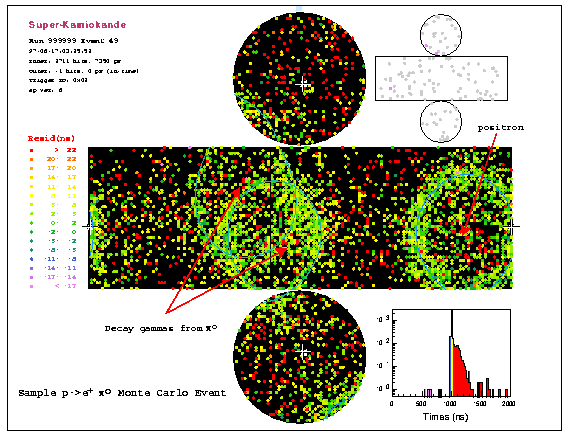
\includegraphics[width=0.8\linewidth]{Figures/epi0_nice_event.png}
    \parencite{boston_university/proton_decay}
\end{frame}


\begin{frame}
    \frametitle{Current limit}

    \begin{itemize}
        \item Running since 1996
        \item No decay observed
            \pause
        \item Lifetime at least \SI{e34}{\year}
        \item Rules out SU(5) GUT
    \end{itemize}

    \parencite{super-k/proton_decay}
\end{frame}

\section{Conclusion}

\begin{frame}
    \frametitle{Conclusion}

    \begin{itemize}
        \item Proton stable in Standard Model
        \item SU(5) GUT predicts decay
        \item Lifetime at least \SI{e34}{\year} \parencite{super-k/proton_decay}
        \item SU(5) GUT ruled out
    \end{itemize}
\end{frame}

%%%%%%%%%%%%%%%%

\section*{End}

\begin{frame}
    \titlepage
\end{frame}

\nocite{tikz-feynman}

\section*{References}

\begin{frame}[allowframebreaks]

    \printbibliography
\end{frame}

\end{document}

% vim: spell spelllang=en_us
